% 5.	I would qualify the claims associated to Table B1 since column (2) shows an estimate twice as large as that in column (1), and column (4) does not allow to reject an ATT equal to zero.

Thanks for the point. We agree that the description of the results of this table (now Table C.1, following the reorganization of the appendices in the revised manuscript) required qualification.

In the previous version of the paper, we wrote the following: ``In this appendix, we estimate the effects of \emph{Plan Cuadrante} on the number of crimes reported to the police and on the total number of arrests, using only the subsample of municipalities included in the analysis of the ENUSC outcomes. While the sample size is smaller, the estimates using this restricted analytical sample, reported in Table B1 and Figure B2, show similar patterns to those observed when using the full sample.''

While the effects on reported crime have the same sign and are statistically significant in both samples, the effects on reported crime are nearly twice as large in the ENUSC sample of municipalities. These municipalities are on average larger and experienced a higher incidence of crime, which may partly explain the larger estimated effect.

Regarding the effects on arrests, the estimates are not statistically significant in the ENUSC sample of municipalities, which is likely due to the smaller sample size. The point estimates are negative and of similar magnitude to those in the full sample, but the standard errors are larger, leading to a failure to reject the null hypothesis of no effect in this sample. 

We have edited the text to reflect these points:

\begin{adjustwidth}{2em}{0em}
In this Online Appendix, we estimate the effects of \emph{Plan Cuadrante} on the number of crimes reported to the police and on the total number of arrests, using only the subsample of municipalities included in the analysis of the ENUSC outcomes. The sample size in this analysis is smaller, and the results are reported in Figure \ref{fig:figure02_N47}. While the effects for reported crime are larger in magnitude and the effects on arrests are not statistically significant in the ENUSC subsample, the estimates are qualitatively similar to those observed in Table \ref{tab:SPD_all_vs_enusc} with the full sample.
\end{adjustwidth}

If the editor or the reviewer feel that this wording should be qualified further, we are happy to do so.

\clearpage
\noindent\textbf{Other figure and table referenced above:}
\vspace{0.5em}

{\renewcommand{\thetable}{C.1}
\begin{table}[h!]
\caption{Effects of \emph{Plan Cuadrante} on Reported Crime and Arrests: Full Sample and ENUSC Municipalities}
\label{tab:SPD_all_vs_enusc}
\begin{center}
\resizebox{12cm}{!}{
\begin{tabular}{lccccccccccccccccccccccccccccccccccccccc} \hline \hline
& & (1) & (2) & (3) & (4) \\
Outcome & & \multicolumn{2}{c}{Reported crime} & \multicolumn{2}{c}{Arrests} \\
\cmidrule(lr){3-4} \cmidrule(lr){5-6}
& & \shortstack{Sample\\Admin} & \shortstack{Sample\\ENUSC} & \shortstack{Sample\\Admin} & \shortstack{Sample\\ENUSC} \\
\cmidrule(lr){3-4} \cmidrule(lr){5-6}
\\
ATT & & -208.02*** & -428.09*** & 48.02*** & 44.09 \\
& & (56.13) & (108.48) & (16.27) & (34.85) \\
\\
N & & 4,231 & 592 & 3,293 & 405 \\
Municipalities & & 292 & 47 & 281 & 40 \\
Y mean & & 2,109.64 & 2,294.96 & 345.65 & 419.61 \\
\hline \hline
\end{tabular}}
\par{
\begin{tabular}{p{12cm}}
\footnotesize{Note: This table shows the effects of \emph{Plan Cuadrante} on the number of crimes reported to the police in the municipality per 100,000 inhabitants and on the number of arrests in the municipality per 100,000 inhabitants using administrative data from the Undersecretary for Crime Prevention. The table reports the results for two samples: the full sample of municipalities included in the administrative database that is used for the analysis of these outcomes and the subsample of these municipalities included in the analysis of ENUSC outcomes. The estimation is conducted using the procedure developed in \citet{Callaway} for difference-in-differences with staggered treatment adoption. Standard errors are clustered at the municipality level using the wild bootstrapping procedure. ***p$<$0.01, **p$<$0.05, *p$<$0.1.} \\
\end{tabular}}
\end{center}
\end{table}
}

\clearpage

{\renewcommand{\thefigure}{C.1}
%--- Implementation
\begin{figure}[h!]
    \centering
    \caption{Effects of \emph{Plan Cuadrante} on Reported Crime and Arrests (Sample of Municipalities Included in the Analysis of ENUSC Outcomes)}
    \label{fig:figure02_N47}
    \begin{subfigure}{0.495\textwidth}
        \centering
        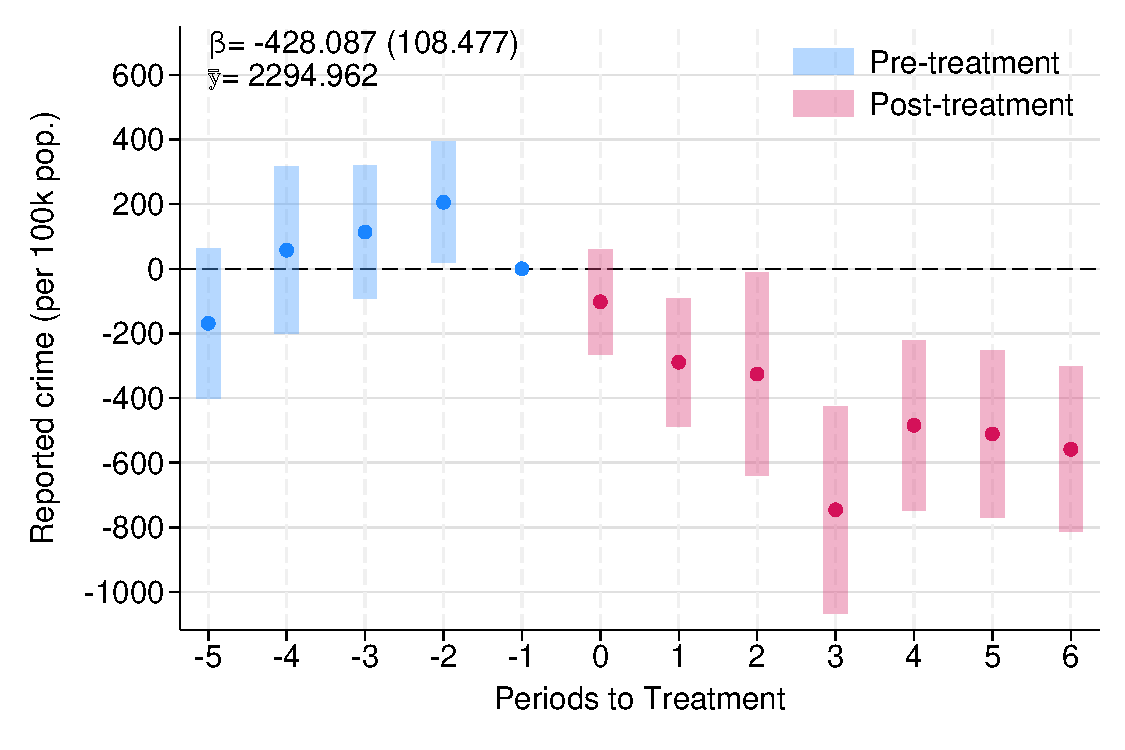
\includegraphics[width=\textwidth]{../manuscript/Graphs/totalreportedcrime_47enusc.pdf}
        \caption{Reported crime per 100k inhabitants}
    \end{subfigure}%
    ~ 
    \begin{subfigure}{0.495\textwidth}
    \centering
    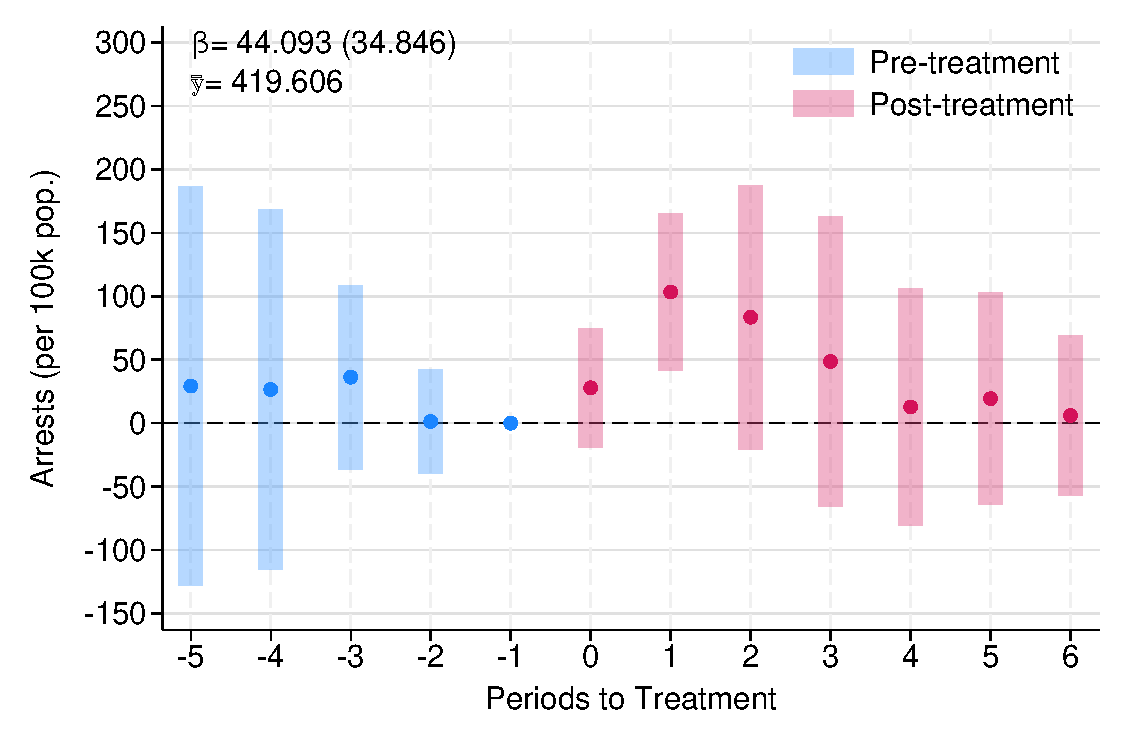
\includegraphics[width=\textwidth]{../manuscript/Graphs/totalarrestscrime_47enusc.pdf}
        \caption{Arrests per 100k inhabitants}
    \end{subfigure}
    \\[12pt]
    \begin{minipage}{0.99\textwidth}
    \footnotesize Notes: This figure shows the dynamic effects of \emph{Plan Cuadrante} on the number of crimes reported to the police per 100,000 inhabitants in the municipality in panel (a) and on the number of arrests per 100,000 inhabitants in the municipality in panel (b) using administrative data from the Undersecretary for Crime Prevention. The analysis is conducted using only the sample of municipalities included in the analysis of ENUSC outcomes. Panel (a) includes 592 observations, while panel (b) includes 405 observations. The estimation is conducted using the procedure developed in \citet{Callaway} for difference-in-differences with staggered treatment adoption. The dots in the figure represent the estimated coefficients and the bars behind them 95\% confidence intervals. Standard errors are clustered at the municipality level using wild bootstrapping. The pooled effect and the mean outcome before the introduction of the treatment is also presented in each panel. 
    \end{minipage}
\end{figure}
}

\clearpage